\chapterimage{unidades/1_computadoras/1_computadoras/imagenes/cover}
\chapterimagedescription{Placa base de una computadora con sus circuitos impresos}
\chapterimageauthor{Fotografía de Blickpixel}

\chapter{Computadoras}

\setcounter{section}{2}
\section{Actividades}
\index{Actividades}

Responda las siguientes preguntas. Puede investigar en Internet si lo cree
conveniente.

\begin{exercise}
Mire el cartel a continuación\\
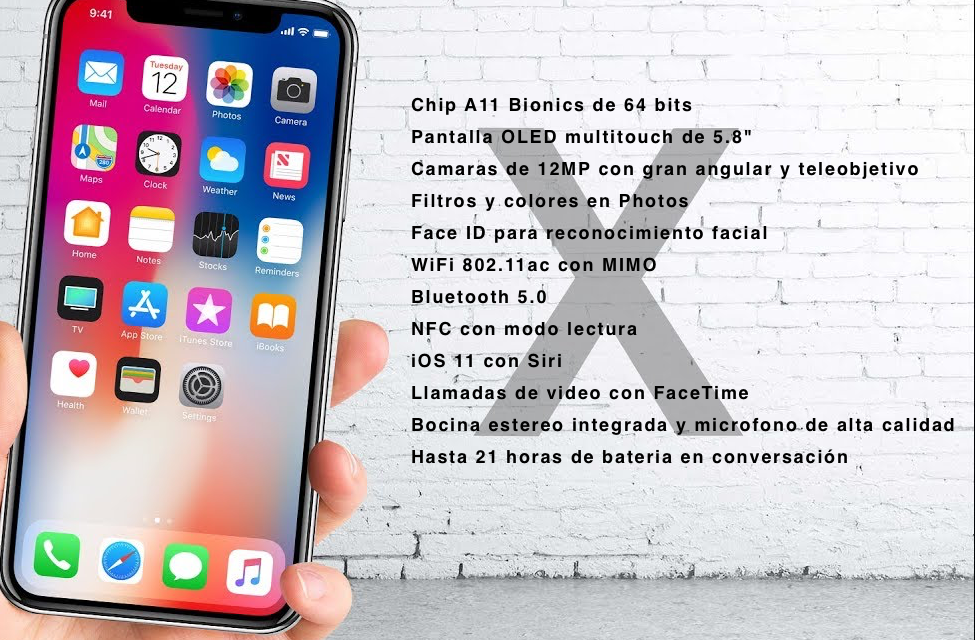
\includegraphics[scale=0.38]{unidades/1_computadoras/1_computadoras/imagenes/iphone_x_specs.png}

Determine.\\
¿Cuáles de los elementos mencionados corresponden a software?\\
¿Cuáles de los elementos mencionados corresponden a hardware?
\end{exercise}

En el cartel, los siguientes elementos aluden directamente al software:

\begin{itemize}
    \item Filtros y colores en Photos
    \item FaceID para reconocimiento facial
    \item iOS 11 con Siri
    \item Llamadas de video con FaceTime
\end{itemize}

Mientras que los siguientes elementos aluden al hardware:

\begin{itemize}
    \item Chip A11 Bionics de 64 bits
    \item Pantalla OLED multitouch de 5.8"
    \item Cámaras de 12MP con gran angular y teleobjetivo
    \item WiFi 802.11ac con MIMO
    \item Bluetooth 5.0
    \item NFC con modo lectura
    \item Bocina estéreo integrada y micrófono de alta calidad
    \item Hasta 21hs de batería en conversación
\end{itemize}

Cada uno de los elementos de hardware requiere de software para funcionar. Por
lo tanto, incluso si refieren a hardware, siempre hay software involucrado para
que el dispositivo funcione y se integre con el sistema operativo. El software
no necesariamente es una aplicación que viene por separado, sino que son partes
especificas del sistema operativo que dar soporte a ese hardware, lo cual se
realiza en forma de firmware, drivers u otros.
\vspace{1cm}

\begin{exercise}
¿Qué sistemas operativos conoce?\\
Discuta su respuesta con compañeros y el docente para descubrir nuevos sistemas.
\end{exercise}


Existen muchos sistemas operativos, algunos ya mencionados en el libro.
Repasemos algunos de ellos, e indagemos sobre otros:

\subsection*{Microsoft Windows}

El más conocido es tal vez \textbf{Microsoft Windows}, debido a que es el
sistema que viene instalado por defecto en muchas computadoras.
\textbf{Microsoft} hizo un acuerdo con la empresa \textbf{IBM}, en donde sus
máquinas se vendían con Windows pre-instalado en sus equipos, que en los 80s y
principios de los 90s eran el estándar de la industria. A medida que aparecían
otros jugadores en la industria del hardware, Microsoft establecía contratos
draconianos para que Windows fuera el sistema por defecto en sus equipos, a la
vez que las empresas de hardware buscaban estos contratos en pos de captar
usuarios ya fieles al sistema operativo de las ventanas.

Microsoft establecería una fuerte campaña de eliminación de la competencia y
monopolio del mercado, al iniciar acuerdos con diversas dependencias del Estado
en las que entregaban Windows de forma gratuita (solo inicialmente), por ejemplo
en el área de educación.

Esto hizo que muchas personas solo hayan sido expuestas a este sistema
operativo, y por tanto es el único que conocen. Peor aún, es el único que saben
manejar, y por tanto, cuando necesitan una nueva computadora, esta debe venir
con Windows (el usuario debe pagar un adicional) o debe instalarse luego (se
debe comprar la licencia).

\image{soluciones/1_computadoras/1_computadoras/imagenes/bliss.jpg}
{Bliss, la imágen de fondo por defecto de Windows XP se ha transformado en un
ícono de ese sistema.} {Imágen de Azuresh.}

Las primeras versiones de Windows estaban basadas en \textbf{MS-DOS}, otro
popular sistema de Microsoft de los 80s. Tuvo varias versiones a lo largo de su
historia, como \textbf{Windows 1.0}, \textbf{Windows 2.0} y \textbf{Windows 3.1}
(Las primeras versiones bastante primitivas, pero que sentaron las bases para
las demás, y donde se desarrolla el concepto de ventana), \textbf{Windows 95}
(El primero en tener el ``botón de inicio''), \textbf{Windows 98} (primero con
soporte para acceso a Internet por defecto), \textbf{Windows NT} (para
computadoras de uso empresarial), \textbf{Windows XP} (el primero en mezclar
tecnologías de NT, con las de 98, que hasta el momento eran tecnologías
separadas. Fue tal vez de las versiones más populares, saliendo en el año 2000),
\textbf{Windows 8} (donde se introdujo la interfaz Metro) y \textbf{Windows 10}
(la versión actual, que mezcla la interfaz Metro con una más tradicional).

\subsection*{MacOS}

Históricamente \textbf{Apple} ha desarrollado sus propios sistemas operativos,
para sus equipos (Ellos se definen como una empresa que vende computadoras, no
sistemas). Las primeras computadoras Apple, como la \textbf{Apple II}, venían
con \textbf{Apple DOS} y luego \textbf{Apple ProDOS}. Más tarde lanzaría lo que
posteriormente se conocería como \textbf{Mac OS}, en ese momento denominado
simplemente \textbf{System}, acompañando su nueva línea de computadoras
Macintosh.

Llegando el 2000, su sistema empezaría a sentir el paso de los años, un nuevo
sistema diseñado desde cero sería lanzado con toda su nueva línea de
computadoras, \textbf{Mac OS X}, sistema que hoy a recibido un rebranding, para
denominarse simplemente \textbf{macOS}, y que acompaña a todas las computadoras
de la marca.

A diferencia de otros sistemas operativos, macOS es un sistema que viene
instalado por defecto en los equipos de Apple, y que no se encuentra disponible
para otros equipos, ni siquiera como compra por separado.


\subsection*{GNU/Linux}

Cuándo inició el movimiento de \textbf{software libre} en 1984, \textbf{Richard
Stallman}, el fundador del movimiento, se propuso realizar un sistema operativo
completamente libre, compatible con \textbf{UNIX} (Un popular sistema de la
época, que era propiedad de AT\&T). Así, Stallman funda el \textbf{Proyecto
GNU}, bajo cuya ala aparecen cientos de herramientas necesarias para el
funcionamiento de un sistema operativo realmente utilizable, como compiladores,
editores, terminales, etc. Sin embargo, el proyecto \textbf{Hurd}, un
sub-proyecto de GNU que desarrollaría el \textbf{núcleo} del sistema operativo,
seguía teniendo cientos de retrasos, idas y vueltas, sin nunca terminar con una
versión utilizable. Ya en 1991, \textbf{Linus Torvalds}, un estudiante de la
Universidad de Helsinki en Finlandia, quería utilizar en su computadora hogareña
un sistema compatible con UNIX. Ante la ausencia de alternativas, se dispuso a
programar su propio sistema, y tras anunciar públicamente en un foro sobre su
desarrollo, Stallman se le acercó para convencerlo de que \textbf{Linux}, nombre
que recibiría el sistema operativo, debía ser libre.

Linux evolucionó, y al ser libre, miles de personas pueden contribuir al
proyecto. Su código es la base para múltiples sistemas operativos empaquetados
para el usuario final, que utilizan el núcleo Linux, junto con las herramientas
de GNU, y otros conjuntos de herramientas, imágenes, iconos, etc. (Lo que se
conoce como una \textbf{distribución}). Hay miles de distribuciones, como
\textbf{Ubuntu}, \textbf{Mint}, \textbf{Fedora}, \textbf{Debian}, \textbf{Arch},
\textbf{Zorin}, \textbf{Huayra}, entre otros tantos. Cualquiera con los
conocimientos técnicos suficientes puede crearse su propia distribución. Lo más
interesante es que existen distintas distribuciones, que se enfocan en distintas
cosas. Así por ejemplo, hay distribuciones para computadoras de escritorios,
otras para teléfonos celulares, otras para grandes servidores, para routers,
para computadoras viejas, para consolas de videojuegos, etc.

\subsection*{BSD}

\image{soluciones/1_computadoras/1_computadoras/imagenes/freebsd.png}
{Imágen de inicio de FreeBSD, corriendo sobre QEMU.} {Imágen de Huihermit.}

Los sistemas \textbf{BSD} (\textbf{Berkley Software Distribution}) comprenden,
al igual que Linux, un núcleo, y varias distribuciones derivadas de dicho núcleo
(Aunque incluso hay núcleos distintos e incompatibles entre si). El sistema
surgió en la \textbf{Universidad de Berkley}, en donde \textbf{Bill Joy} compiló
un conjunto de programas creados en la universidad que corrían sobre la versión
6 de UNIX. Otros universidades que utilizaban UNIX, podían entonces instalar
dichos programas en sus computadoras. Los programas comenzaron a crecer y a
incluir cambios en el mismo sistema UNIX. Sin embargo, por ser solo
modificaciones a partes del sistema, aunque Berkley distribuía todo el sistema
UNIX modificado, AT\&T seguía siendo el dueño del sistema, y por tanto, quien
quisiera utilizarlo debía pagar a AT\&T.

Tras una disputa legal que tomaría años resolver, Berkley dejaría de distribuir
el software. Tras la resolución del conflicto en 1992, y tras quitar todo rastro
de código del sistema UNIX original, se liberaría \textbf{BSD 4.2}. Berkley
distribuye el sistema bajo una licencia llamada \textbf{Licencia BSD}, que
permite que cualquiera pueda tomar el código de BSD y utilizarlo para lo que
quiera, inclusive, en proyectos comerciales de código cerrado.

Hoy hay varias distribuciones BSD, como \textbf{FreeBSD}, \textbf{OpenBSD}, y
\textbf{NetBSD}, pero hay muchas otras a su vez derivadas de estas tres. No solo
eso sino que \textbf{parte del código de BSD se encuentra en Windows}, y
\textbf{es la base para macOS de Apple}.

\subsection*{iOS}

\textbf{iOS} es un sistema operativo creado por \textbf{Apple} para que corra de
forma exclusiva en el \textbf{iPhone} y luego en \textbf{iPad}. El sistema
utiliza una gran cantidad de código de BSD, y también de macOS.

Este sistema se crea pensando en la optimización de recursos y de batería, así
como en una interfaz que pueda ser utilizada de forma sencilla en un dispositivo
que no cuenta ni con teclado ni mouse.

\subsection*{Android}

\textbf{Android} es un sistema creado por \textbf{Google}, basándose en el
núcleo de \textbf{Linux} (Aunque el mismo está altamente modificado para
funcionar de forma óptima en dispositivos móviles y tablets). El sistema, al
estar basado en Linux es software libre, pero la mayoría de los fabricantes de
teléfonos que venden dispositivos con Linux agregan gran cantidad de
herramientas no libres sobre el sistema, comenzando por \textbf{Google}, que
incluye no solo \textbf{Play Store}, sino también aplicaciones como
\textbf{Gmail}, \textbf{Calendar}, etc.

\subsection*{Otros sistemas}

Estos no son los únicos sistemas operativos. Existen cientos, y siempre aparecen
nuevos (Aunque muchos son altamente experimentales, o son solo prototipos que
fracasan). Ejemplos interesantes son \textbf{ReactOS} (Un sistema libre que
intenta generar un sistema completamente compatible con Windows XP),
\textbf{Haiku} (Un sistema que intenta revivir BeOS, y ser compatible con este),
\textbf{MenuetOS} (Un sistema operativo que pesa solo 3.25MB) y \textbf{Plan9}
(Un sistema operativo experimental de Bell Labs).

A lo largo de la historia han habido varios otros sistemas que han ganados
varios adeptos, y cuyas ideas innovadoras en muchos casos fueron luego adoptadas
por los sistemas comerciales más grandes, como \textbf{Amiga OS}, \textbf{BeOS},
\textbf{Symbian}, entre otros.

Finalmente podemos mencionar que existen sistemas operativos mucho más oscuros,
experimentales y casi sin usuarios. Un caso muy interesante es el
\textbf{TempleOS}, un sistema operativo con contenidos bíblicos, creado por
Terry A. Davis, quien lo creó con la intensión de transformar al sistema
operativo en el tercer templo profetizado en la biblia. Davis comenzó a sufrir
una serie de epizodios esquizofrénicos y alusinaciones sobre invasiones
extraterrestres y conspiraciones gubernamentales, motivo por el cual estuvo
hospitalizado en reiteradas ocasiones. Tras una autoproclamada ``revelación''
hacia su persona por Diós, con quien él dice tener comunicación directa, comenzó
el trabajo de desarrollar dicho sistema operativo, pues consideraba a otros
sistemas como impuros y llenos de pecado. TempleOS ha sido criticado por
expertos como una excelente pieza de ingeniería y un trabajo excelente para ser
producto de una sola persona, aunque no sea un sistema operativo capaz de ser
utilizado para el día a día.
\vspace{1cm}

\begin{exercise}
¿Se le ocurren otros dispositivos de hardware que use de forma cotidiana?\\
¿Son periféricos de entrada, de salida, de entrada y salida, o de
almacenamiento?
\end{exercise}

Existen cientos de dispositivos. Por ejemplo, como entrada es común encontrar
emisores infrarrojos. Esto es fácil de encontrar en consolas de videojuegos
(Zappers, Control de Wii, entre otros). También son comunes los sensores de
presión (Botones táctiles, o plataformas sobre las cuales uno se puede parar).

En la parte de salida, existen diversas cosas, como rotores y motores que pueden
generar movimiento, abriendo o cerrando tuberías u otros. También hay incluso
proyectores holográficos.

